\section{Game Playing}
\label{s:gamePlaying}
\chapterquote{Het is geen schande gespeeld te hebben, maar wel om geen einde te maken aan het spel.}{Horatius, Romeins dichter (65 v.C. - 8 v.C.)}
Een andere tak van de Artifici\"ele intelligentie is \termen{Game Playing}. Dit probleem is net als Constraint-Processing een speciaal geval van zoekproblemen die speciale eisen stelt. Game Playing stelt ons verder ook in staat Artifici\"ele systemen te beoordelen. Dit komt omdat spelletjes zich meestal heel goed lenen tot State-Spaces: De regels zijn zeer duidelijk (ze worden zelf opgesteld, soms in tegenstelling tot de echte wereld) en er is makkelijk een representatie voor te bedenken.
\paragraph{Indeling van games}
We kunnen games indelen met behulp van twee parameters:
\begin{itemize}
 \item Determinisme: is er een kans-element in het spel of niet
 \item Informatie Symmetrie: indien alle spelers even veel weten spreken we van ``Perfecte Informatie'' (voorbeeld: Schaken), Bij ``Inperfecte Informatie'' kennen de spelers slechts een deel van de informatie in het spel. (voorbeeld: Poker, Stratego).
\end{itemize}
\paragraph{Waarom zijn nieuwe technieken vereist?}
Er zijn twee grote problemen waarom zoekalgoritmen meestal niet goed werken:
\begin{itemize}
 \item Het \termen{``Contingency'' probleem}\footnote{Voor meer hierover: zie publicaties van John Nash over het ``Nash-evenwicht''}: Verschillende spelers hebben tegenstrijdige belangen, de ene speler stelt een andere doel dan de andere speler, bovendien zal de tegenstander niet noodzakelijk de voor hem beste zet doen.
 \item De grote van het zoekprobleem: Spelletjes zijn er meestal op gericht er voor te zorgen dat zoeken onmogelijk is. Een voorbeeld is schaken waar de vertakkingsfactor gemiddeld $b=15$ is en de diepte zo'n $d=80$ zetten. Dit leidt dus tot $b^d=15^{80}\approx1.223\times10^{94}$ knopen, geen enkele hedendaagse machine is in staat een dergelijke boom binnen een redelijke tijd af te zoeken.
\end{itemize}
De oplossing bestaan er dan ook uit om bomen slechts tot een bepaalde diepte te onderzoeken, vanaf de huidige toestand. Door middel van een \termen{evaluatie-functie} $\mathfunc{eval}{S}$ wordt vervolgens de situatie beoordeeld. Dit oordeel wordt vervolgens naar boven gepropageerd in de boom, waardoor we bij iedere knoop op het eerste niveau een waarde bekomen. Afhankelijk van deze waarden kunnen we vervolgens een keuze maken.
\subsection{Leidend Voorbeeld: Tic-Tac-Toe}
\begin{leftbar}
Als voorbeeld zullen we het Tic-Tac-Toe spel bespreken. Dit spel, ook wel ``Boter, kaas en Eieren'' genoemd wordt gespeeld op een $3\times3$ bord. De spelers dienen beurtelings respectievelijk een kruis of cirkel op het bord plaatsen. Bedoeling is drie van de eigen tekens op \'e\'en lijn te plaatsen. Dit spel is eenvoudig voor pedagogische voorbeelden omdat de regels simpel zijn, en het spel beperkt is tot 765 mogelijke bordposities. Een mogelijk spelverloop beschrijven we of figuur \ref{fig:ticTacToeExample}.
\end{leftbar}
\begin{figure}[htb]
\centering
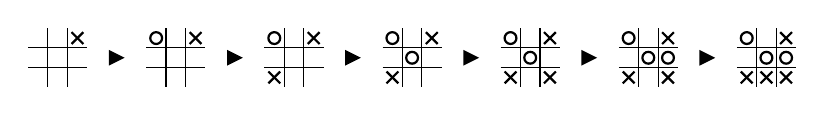
\begin{tikzpicture}
\def\da{0.1};
\def\ds{1.5};
\def\dm{0.375};
\def\dx{0.25};
\def\dr{0.075};
\foreach\s in {0,1,...,5} {
  \fill (\ds+\s*\ds+\da,0) -- (\ds+\s*\ds-\da,\da) -- (\ds+\s*\ds-\da,-\da) -- cycle;
}
\foreach\s in {0,1,...,6} {
  \draw (\dm+\s*\ds,0.5*\dx) -- (\ds-\dm+\s*\ds,0.5*\dx);
  \draw (\dm+\s*\ds,-0.5*\dx) -- (\ds-\dm+\s*\ds,-0.5*\dx);
  \draw (\ds*\s+0.5*\ds-0.5*\dx,0.5*\ds-\dm) -- (\ds*\s+0.5*\ds-0.5*\dx,-0.5*\ds+\dm);
  \draw (\ds*\s+0.5*\ds+0.5*\dx,0.5*\ds-\dm) -- (\ds*\s+0.5*\ds+0.5*\dx,-0.5*\ds+\dm);
}
%circles
\foreach\s/\x/\y in {1/0/2,2/0/2,3/0/2,3/1/1,4/0/2,4/1/1,5/0/2,5/1/1,5/2/1,6/0/2,6/1/1,6/2/1} {
  \draw[thick] (\ds*\s+\dm+\dx*\x+0.5*\dx,\dx*\y-\dx) circle (\dr);
}
%crosses
\foreach\s/\x/\y in {0/2/2,1/2/2,2/2/2,2/0/0,3/2/2,3/0/0,4/2/2,4/0/0,4/2/0,5/2/2,5/0/0,5/2/0,6/2/2,6/0/0,6/2/0,6/1/0} {
  \draw[thick] (\ds*\s+\dm+\dx*\x+0.5*\dx-\dr,\dx*\y-\dx-\dr) -- (\ds*\s+\dm+\dx*\x+0.5*\dx+\dr,\dx*\y-\dx+\dr);
  \draw[thick] (\ds*\s+\dm+\dx*\x+0.5*\dx-\dr,\dx*\y-\dx+\dr) -- (\ds*\s+\dm+\dx*\x+0.5*\dx+\dr,\dx*\y-\dx-\dr);
}
\end{tikzpicture}
\caption{Een mogelijk spelscenario bij Tic-Tac-Toe}
\label{fig:ticTacToeExample}
\end{figure}
\begin{leftbar}
We zullen in onze experimenten met dit voorbeeld geroteerde situaties als equivalent beschouwen. Borden die dus door enkele rotaties van 90 graden gelijk aan elkaar zijn beschouwen we als equivalent. Daarnaast worden ook spiegelingen over het middelste vak (horizontaal en verticaal op de tweede rij, kolom of diagonaal) op dezelfde manier behandeld. Dit is redelijk omdat de rotatie en diagonale spiegeling bij dit spel geen enkele rol speelt. Dit illustreren we in figuur \ref{fig:ticTacToeEquivalent}.
\end{leftbar}
\begin{figure}[htb]
\centering
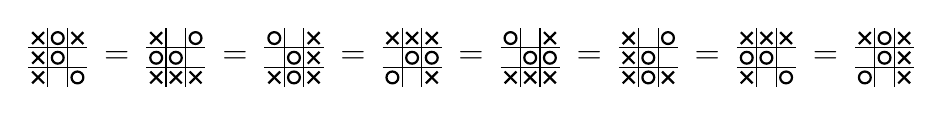
\begin{tikzpicture}
\def\da{0.1};
\def\ds{1.5};
\def\dm{0.375};
\def\dx{0.25};
\def\dr{0.075};
\foreach\s in {0,1,...,6} {
  \draw (\ds+\s*\ds,0) node {\large $=$};
}
\foreach\s in {0,1,...,7} {
  \draw (\dm+\s*\ds,0.5*\dx) -- (\ds-\dm+\s*\ds,0.5*\dx);
  \draw (\dm+\s*\ds,-0.5*\dx) -- (\ds-\dm+\s*\ds,-0.5*\dx);
  \draw (\ds*\s+0.5*\ds-0.5*\dx,0.5*\ds-\dm) -- (\ds*\s+0.5*\ds-0.5*\dx,-0.5*\ds+\dm);
  \draw (\ds*\s+0.5*\ds+0.5*\dx,0.5*\ds-\dm) -- (\ds*\s+0.5*\ds+0.5*\dx,-0.5*\ds+\dm);
}
%circles
\foreach\s/\x/\y in {0/1/1,0/1/2,0/2/0,1/0/1,1/1/1,1/2/2,2/1/0,2/0/2,2/1/1,3/2/1,3/0/0,3/1/1,4/2/1,4/0/2,4/1/1,5/1/1,5/1/0,5/2/2,6/1/1,6/2/0,6/0/1,7/1/1,7/1/2,7/0/0} {
  \draw[thick] (\ds*\s+\dm+\dx*\x+0.5*\dx,\dx*\y-\dx) circle (\dr);
}
%crosses
\foreach\s/\x/\y in {0/0/0,0/0/1,0/0/2,0/2/2,1/0/0,1/1/0,1/2/0,1/0/2,2/0/0,2/2/2,2/2/0,2/2/1,3/1/2,3/2/0,3/0/2,3/2/2,4/2/2,4/0/0,4/2/0,4/1/0,5/0/0,5/0/1,5/0/2,5/2/0,6/0/2,6/1/2,6/2/2,6/0/0,7/2/0,7/2/1,7/2/2,7/0/2} {
  \draw[thick] (\ds*\s+\dm+\dx*\x+0.5*\dx-\dr,\dx*\y-\dx-\dr) -- (\ds*\s+\dm+\dx*\x+0.5*\dx+\dr,\dx*\y-\dx+\dr);
  \draw[thick] (\ds*\s+\dm+\dx*\x+0.5*\dx-\dr,\dx*\y-\dx+\dr) -- (\ds*\s+\dm+\dx*\x+0.5*\dx+\dr,\dx*\y-\dx-\dr);
}
\end{tikzpicture}
\caption{Equivalente situaties bij Tic-Tac-Toe}
\label{fig:ticTacToeEquivalent}
\end{figure}
\begin{leftbar}
We hebben nood aan een evaluatie-functie om een bepaalde toestand te evalueren. De drijvende kracht achter Tic-Tac-Toe zijn de verschillende lijnen. We berekenen dus voor elke lijn een bepaalde score. De evaluatie-functie is vervolgens de som van de score van de 8 lijnen. Een lijn krijgt een score $0$ indien deze zowel een kruis als cirkel bevat. Indien enkel \'e\'en soort tekens aanwezig is, geven we de lijn een score afhankelijk van het aantal: $l(n)=10^{n-1}$. We nemen $X$ als het positieve teken, en $O$ als het negatieve teken.
\end{leftbar}
\subsection{Mini-Max}
De propagatie naar boven in de boom verloopt volgens het \termen{Mini-Max}-principe. Hierbij gaan we ervan uit dat de computer de situatie beoordeelt, volgens hoe goed hij er zelf voor staat. De computer streeft met andere woorden naar een zo maximaal mogelijke evaluatie. De tegenstander anderzijds streeft naar een zo laag mogelijke evaluatie. Dit resulteert in het feit dat bij een knoop waar de computer een keuze dient te maken, hij de maximale waarde verder naar boven zal propageren. De tegenstander daarentegen zal de minimale evaluatie van zijn kinderen overnemen. Dit idee wordt formeel weergegeven in \algref{alg:minimax}, waarbij we de methode initieel aanroepen met $\depth=0$ en $\mbox{board}$ met de huidige staat van het bord.
\begin{algorithm}[htb]                      % enter the algorithm environment
\caption{$\mathcommand{minimax}{\mbox{board},\depth}$}          % give the algorithm a caption
\label{alg:minimax}                           % and a label for \ref{} commands later in the document
\begin{algorithmic}[1]                    % enter the algorithmic environment
\IF{$\depth<\depthbound$}
\STATE\COMMENT{Einde nog niet bereikt}
\IF{$\mathcommand{isMaxLevel}{\depth}$}
\STATE$M\leftarrow-\infty$
\FORALL{$c\in\mathcommand{children}{\mbox{board}}$}
\STATE M=\maxM{}{M,\mathcommand{minimax}{c,\depth+1}}
\ENDFOR
\RETURN $M$
\ELSE
\STATE$m\leftarrow\infty$
\FORALL{$c\in\mathcommand{children}{\mbox{board}}$}
\STATE m=\minM{}{m,\mathcommand{minimax}{c,\depth+1}}
\ENDFOR
\RETURN $m$
\ENDIF
\ELSE
\STATE\COMMENT{Eind-diepte bereikt}
\RETURN $\mathcommand{eval}{\mbox{board}}$
\ENDIF
\end{algorithmic}
\end{algorithm}
\begin{leftbar}
We kunnen nu een boom opstellen die het Mini-Max principe illustreert bij Tic-Tac-Toe voor een diepte $d=2$. Waarbij we ook de propagatie naar boven toe tonen. Rechtsboven ieder bord tonen we de evaluatiefunctie toegepast op dit bord. Onder ieder bord, staat de gepropageerde waarde. Volgens deze boom is het plaatsen van een $X$ in het midden de beste zet.
\end{leftbar}
% \begin{figure}[htb]
% \centering
% \begin{tikzpicture}
% \def\dy{-1.75};
% \def\dx{1.25};
% \def\l{0.87};
% \def\s{0.29};%\l/3
% \def\r{0.2};
% \draw (-0.5*\l,0.5*\s) -- (0.5*\l,0.5*\s);
% \draw (-0.5*\l,-0.5*\s) -- (0.5*\l,-0.5*\s);
% \draw (-0.5*\s,0.5*\l) -- (-0.5*\s,-0.5*\l);
% \draw (0.5*\s,-0.5*\l) -- (0.5*\s,0.5*\l);
% \foreach\x/\xxa/\yxa in {-3.5/0/2,1.5/1/2,5/1/1} {
%   \draw (-0.5*\l+\dx*\x,0.5*\s+\dy) -- (0.5*\l+\dx*\x,0.5*\s+\dy);
%   \draw (-0.5*\l+\dx*\x,-0.5*\s+\dy) -- (0.5*\l+\dx*\x,-0.5*\s+\dy);
%   \draw (-0.5*\s+\dx*\x,0.5*\l+\dy) -- (-0.5*\s+\dx*\x,-0.5*\l+\dy);
%   \draw (0.5*\s+\dx*\x,-0.5*\l+\dy) -- (0.5*\s+\dx*\x,0.5*\l+\dy);
%   \draw[thick] (\s*\xxa-\s-0.5*\r+\dx*\x,\s*\yxa-\s-0.5*\r+\dy) -- (\s*\xxa-\s+0.5*\r+\dx*\x,\s*\yxa-\s+0.5*\r+\dy);
%   \draw[thick] (\s*\xxa-\s+0.5*\r+\dx*\x,\s*\yxa-\s-0.5*\r+\dy) -- (\s*\xxa-\s-0.5*\r+\dx*\x,\s*\yxa-\s+0.5*\r+\dy);
% %  \draw[thick] (+\dx*\x,+\dy) -- (+\dx*\x,+\dy);
% }%(+\dx*\x,+\dy)
% \foreach\x/\xxa/\yxa/\xoa/\yoa in {-5.5/0/2/0/1,-4.5/0/2/1/1,-3.5/0/2/0/0,-2.5/0/2/1/0,-1.5/0/2/2/0,-0.5/1/2/0/2,0.5/1/2/0/1,1.5/1/2/1/1,2.5/1/2/0/0,3.5/1/2/1/0,4.5/1/1/0/2,5.5/1/1/1/2} {
%   \draw (-0.5*\l+\dx*\x,0.5*\s+2*\dy) -- (0.5*\l+\dx*\x,0.5*\s+2*\dy);
%   \draw (-0.5*\l+\dx*\x,-0.5*\s+2*\dy) -- (0.5*\l+\dx*\x,-0.5*\s+2*\dy);
%   \draw (-0.5*\s+\dx*\x,0.5*\l+2*\dy) -- (-0.5*\s+\dx*\x,-0.5*\l+2*\dy);
%   \draw (0.5*\s+\dx*\x,-0.5*\l+2*\dy) -- (0.5*\s+\dx*\x,0.5*\l+2*\dy);
%   \draw[thick] (\s*\xxa-\s-0.5*\r+\dx*\x,\s*\yxa-\s-0.5*\r+2*\dy) -- (\s*\xxa-\s+0.5*\r+\dx*\x,\s*\yxa-\s+0.5*\r+2*\dy);
%   \draw[thick] (\s*\xxa-\s+0.5*\r+\dx*\x,\s*\yxa-\s-0.5*\r+2*\dy) -- (\s*\xxa-\s-0.5*\r+\dx*\x,\s*\yxa-\s+0.5*\r+2*\dy);
%   \draw[thick] (\s*\xoa-\s+\dx*\x,\s*\yoa-\s+2*\dy) circle(0.5*\r);
% %  \draw[thick] (+\dx*\x,+\dy) -- (+\dx*\x,+\dy);
% }%(+\dx*\x,+\dy)
% \end{tikzpicture}
% \caption{Mini-Max boom van Tic-Tac-Toe}
% \label{fig:miniMaxTicTacToe}
% \end{figure}
\begin{figure}[htb]
\centering
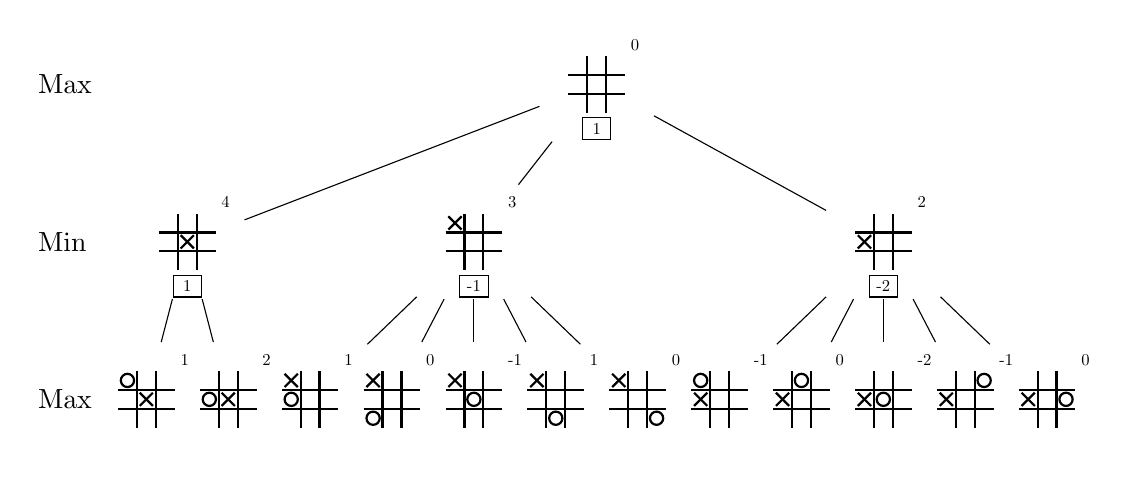
\begin{tikzpicture}[board/.style={minimum width=12*\s cm,minimum height=12*\s cm},eval/.style={anchor=south west,scale=5*\s},minmax/.style={draw=black,rectangle,anchor=north,scale=5*\s,minimum width=5*\s cm}]
\def\s{0.12};
\def\dx{1.04 cm};
\def\dy{-2 cm};
\draw (-1.5,0) node[anchor=west]{Max};
\draw (-1.5,\dy) node[anchor=west]{Min};
\draw (-1.5,2*\dy) node[anchor=west]{Max};

\node[board] (S) at (5.5*\dx,0) {};
\node[board] (SA) at (0.5*\dx,\dy) {};
\node[board] (SAA) at (0,2*\dy) {};
\node[board] (SAB) at (\dx,2*\dy) {};
\node[board] (SB) at (4*\dx,\dy) {};
\node[board] (SBA) at (2*\dx,2*\dy) {};
\node[board] (SBB) at (3*\dx,2*\dy) {};
\node[board] (SBC) at (4*\dx,2*\dy) {};
\node[board] (SBD) at (5*\dx,2*\dy) {};
\node[board] (SBE) at (6*\dx,2*\dy) {};
\node[board] (SC) at (9*\dx,\dy) {};
\node[board] (SCA) at (7*\dx,2*\dy) {};
\node[board] (SCB) at (8*\dx,2*\dy) {};
\node[board] (SCC) at (9*\dx,2*\dy) {};
\node[board] (SCD) at (10*\dx,2*\dy) {};
\node[board] (SCE) at (11*\dx,2*\dy) {};

\draw (S) -- (SA);
\draw (SA) -- (SAA);
\draw (SA) -- (SAB);
\draw (S) -- (SB);
\draw (SB) -- (SBA);
\draw (SB) -- (SBB);
\draw (SB) -- (SBC);
\draw (SB) -- (SBD);
\draw (SB) -- (SBE);
\draw (S) -- (SC);
\draw (SC) -- (SCA);
\draw (SC) -- (SCB);
\draw (SC) -- (SCC);
\draw (SC) -- (SCD);
\draw (SC) -- (SCE);

\begin{scope}[xshift=5.5*\dx,yshift=0]
 \draw[thick] (-3*\s,-\s) -- (3*\s,-\s);
 \draw[thick] (-3*\s,\s) -- (3*\s,\s);
 \draw[thick] (-\s,-3*\s) -- (-\s,3*\s);
 \draw[thick] (\s,-3*\s) -- (\s,3*\s);
 \draw (3*\s,3*\s) node[eval]{0};
 \draw (0,-3.5*\s) node[minmax]{1};
\end{scope}

\begin{scope}[xshift=0.5*\dx,yshift=\dy]
 \draw[thick] (-3*\s,-\s) -- (3*\s,-\s);
 \draw[thick] (-3*\s,\s) -- (3*\s,\s);
 \draw[thick] (-\s,-3*\s) -- (-\s,3*\s);
 \draw[thick] (\s,-3*\s) -- (\s,3*\s);
 \draw (3*\s,3*\s) node[eval]{4};
 \foreach\x/\y in {0/0} {
  \draw[thick] (-0.7*\s+2*\s*\x,-0.7*\s-2*\s*\y) -- (0.7*\s+2*\s*\x,0.7*\s-2*\s*\y);
  \draw[thick] (0.7*\s+2*\s*\x,-0.7*\s-2*\s*\y) -- (-0.7*\s+2*\s*\x,0.7*\s-2*\s*\y);
 }
 \draw (0,-3.5*\s) node[minmax]{1};
\end{scope}
\begin{scope}[xshift=4*\dx,yshift=\dy]
 \draw[thick] (-3*\s,-\s) -- (3*\s,-\s);
 \draw[thick] (-3*\s,\s) -- (3*\s,\s);
 \draw[thick] (-\s,-3*\s) -- (-\s,3*\s);
 \draw[thick] (\s,-3*\s) -- (\s,3*\s);
 \draw (3*\s,3*\s) node[eval]{3};
 \foreach\x/\y in {-1/-1} {
  \draw[thick] (-0.7*\s+2*\s*\x,-0.7*\s-2*\s*\y) -- (0.7*\s+2*\s*\x,0.7*\s-2*\s*\y);
  \draw[thick] (0.7*\s+2*\s*\x,-0.7*\s-2*\s*\y) -- (-0.7*\s+2*\s*\x,0.7*\s-2*\s*\y);
 }
 \draw (0,-3.5*\s) node[minmax]{-1};
\end{scope}
\begin{scope}[xshift=9*\dx,yshift=\dy]
 \draw[thick] (-3*\s,-\s) -- (3*\s,-\s);
 \draw[thick] (-3*\s,\s) -- (3*\s,\s);
 \draw[thick] (-\s,-3*\s) -- (-\s,3*\s);
 \draw[thick] (\s,-3*\s) -- (\s,3*\s);
 \draw (3*\s,3*\s) node[eval]{2};
 \foreach\x/\y in {-1/0} {
  \draw[thick] (-0.7*\s+2*\s*\x,-0.7*\s-2*\s*\y) -- (0.7*\s+2*\s*\x,0.7*\s-2*\s*\y);
  \draw[thick] (0.7*\s+2*\s*\x,-0.7*\s-2*\s*\y) -- (-0.7*\s+2*\s*\x,0.7*\s-2*\s*\y);
 }
 \draw (0,-3.5*\s) node[minmax]{-2};
\end{scope}

\begin{scope}[xshift=0,yshift=2*\dy]
 \draw[thick] (-3*\s,-\s) -- (3*\s,-\s);
 \draw[thick] (-3*\s,\s) -- (3*\s,\s);
 \draw[thick] (-\s,-3*\s) -- (-\s,3*\s);
 \draw[thick] (\s,-3*\s) -- (\s,3*\s);
 \draw (3*\s,3*\s) node[eval]{1};
 \foreach\x/\y in {0/0} {
  \draw[thick] (-0.7*\s+2*\s*\x,-0.7*\s-2*\s*\y) -- (0.7*\s+2*\s*\x,0.7*\s-2*\s*\y);
  \draw[thick] (0.7*\s+2*\s*\x,-0.7*\s-2*\s*\y) -- (-0.7*\s+2*\s*\x,0.7*\s-2*\s*\y);
 }
 \foreach\x/\y in {-1/-1} {
  \draw[thick] (2*\s*\x,-2*\s*\y) circle (0.7*\s);
 }
\end{scope}
\begin{scope}[xshift=1*\dx,yshift=2*\dy]
 \draw[thick] (-3*\s,-\s) -- (3*\s,-\s);
 \draw[thick] (-3*\s,\s) -- (3*\s,\s);
 \draw[thick] (-\s,-3*\s) -- (-\s,3*\s);
 \draw[thick] (\s,-3*\s) -- (\s,3*\s);
 \draw (3*\s,3*\s) node[eval]{2};
 \foreach\x/\y in {0/0} {
  \draw[thick] (-0.7*\s+2*\s*\x,-0.7*\s-2*\s*\y) -- (0.7*\s+2*\s*\x,0.7*\s-2*\s*\y);
  \draw[thick] (0.7*\s+2*\s*\x,-0.7*\s-2*\s*\y) -- (-0.7*\s+2*\s*\x,0.7*\s-2*\s*\y);
 }
 \foreach\x/\y in {-1/0} {
  \draw[thick] (2*\s*\x,-2*\s*\y) circle (0.7*\s);
 }
\end{scope}
\begin{scope}[xshift=2*\dx,yshift=2*\dy]
 \draw[thick] (-3*\s,-\s) -- (3*\s,-\s);
 \draw[thick] (-3*\s,\s) -- (3*\s,\s);
 \draw[thick] (-\s,-3*\s) -- (-\s,3*\s);
 \draw[thick] (\s,-3*\s) -- (\s,3*\s);
 \draw (3*\s,3*\s) node[eval]{1};
 \foreach\x/\y in {-1/-1} {
  \draw[thick] (-0.7*\s+2*\s*\x,-0.7*\s-2*\s*\y) -- (0.7*\s+2*\s*\x,0.7*\s-2*\s*\y);
  \draw[thick] (0.7*\s+2*\s*\x,-0.7*\s-2*\s*\y) -- (-0.7*\s+2*\s*\x,0.7*\s-2*\s*\y);
 }
 \foreach\x/\y in {-1/0} {
  \draw[thick] (2*\s*\x,-2*\s*\y) circle (0.7*\s);
 }
\end{scope}
\begin{scope}[xshift=3*\dx,yshift=2*\dy]
 \draw[thick] (-3*\s,-\s) -- (3*\s,-\s);
 \draw[thick] (-3*\s,\s) -- (3*\s,\s);
 \draw[thick] (-\s,-3*\s) -- (-\s,3*\s);
 \draw[thick] (\s,-3*\s) -- (\s,3*\s);
 \draw (3*\s,3*\s) node[eval]{0};
 \foreach\x/\y in {-1/-1} {
  \draw[thick] (-0.7*\s+2*\s*\x,-0.7*\s-2*\s*\y) -- (0.7*\s+2*\s*\x,0.7*\s-2*\s*\y);
  \draw[thick] (0.7*\s+2*\s*\x,-0.7*\s-2*\s*\y) -- (-0.7*\s+2*\s*\x,0.7*\s-2*\s*\y);
 }
 \foreach\x/\y in {-1/1} {
  \draw[thick] (2*\s*\x,-2*\s*\y) circle (0.7*\s);
 }
\end{scope}
\begin{scope}[xshift=4*\dx,yshift=2*\dy]
 \draw[thick] (-3*\s,-\s) -- (3*\s,-\s);
 \draw[thick] (-3*\s,\s) -- (3*\s,\s);
 \draw[thick] (-\s,-3*\s) -- (-\s,3*\s);
 \draw[thick] (\s,-3*\s) -- (\s,3*\s);
 \draw (3*\s,3*\s) node[eval]{-1};
 \foreach\x/\y in {-1/-1} {
  \draw[thick] (-0.7*\s+2*\s*\x,-0.7*\s-2*\s*\y) -- (0.7*\s+2*\s*\x,0.7*\s-2*\s*\y);
  \draw[thick] (0.7*\s+2*\s*\x,-0.7*\s-2*\s*\y) -- (-0.7*\s+2*\s*\x,0.7*\s-2*\s*\y);
 }
 \foreach\x/\y in {0/0} {
  \draw[thick] (2*\s*\x,-2*\s*\y) circle (0.7*\s);
 }
\end{scope}
\begin{scope}[xshift=5*\dx,yshift=2*\dy]
 \draw[thick] (-3*\s,-\s) -- (3*\s,-\s);
 \draw[thick] (-3*\s,\s) -- (3*\s,\s);
 \draw[thick] (-\s,-3*\s) -- (-\s,3*\s);
 \draw[thick] (\s,-3*\s) -- (\s,3*\s);
 \draw (3*\s,3*\s) node[eval]{1};
 \foreach\x/\y in {-1/-1} {
  \draw[thick] (-0.7*\s+2*\s*\x,-0.7*\s-2*\s*\y) -- (0.7*\s+2*\s*\x,0.7*\s-2*\s*\y);
  \draw[thick] (0.7*\s+2*\s*\x,-0.7*\s-2*\s*\y) -- (-0.7*\s+2*\s*\x,0.7*\s-2*\s*\y);
 }
 \foreach\x/\y in {0/1} {
  \draw[thick] (2*\s*\x,-2*\s*\y) circle (0.7*\s);
 }
\end{scope}
\begin{scope}[xshift=6*\dx,yshift=2*\dy]
 \draw[thick] (-3*\s,-\s) -- (3*\s,-\s);
 \draw[thick] (-3*\s,\s) -- (3*\s,\s);
 \draw[thick] (-\s,-3*\s) -- (-\s,3*\s);
 \draw[thick] (\s,-3*\s) -- (\s,3*\s);
 \draw (3*\s,3*\s) node[eval]{0};
 \foreach\x/\y in {-1/-1} {
  \draw[thick] (-0.7*\s+2*\s*\x,-0.7*\s-2*\s*\y) -- (0.7*\s+2*\s*\x,0.7*\s-2*\s*\y);
  \draw[thick] (0.7*\s+2*\s*\x,-0.7*\s-2*\s*\y) -- (-0.7*\s+2*\s*\x,0.7*\s-2*\s*\y);
 }
 \foreach\x/\y in {1/1} {
  \draw[thick] (2*\s*\x,-2*\s*\y) circle (0.7*\s);
 }
\end{scope}
\begin{scope}[xshift=7*\dx,yshift=2*\dy]
 \draw[thick] (-3*\s,-\s) -- (3*\s,-\s);
 \draw[thick] (-3*\s,\s) -- (3*\s,\s);
 \draw[thick] (-\s,-3*\s) -- (-\s,3*\s);
 \draw[thick] (\s,-3*\s) -- (\s,3*\s);
 \draw (3*\s,3*\s) node[eval]{-1};
 \foreach\x/\y in {-1/0} {
  \draw[thick] (-0.7*\s+2*\s*\x,-0.7*\s-2*\s*\y) -- (0.7*\s+2*\s*\x,0.7*\s-2*\s*\y);
  \draw[thick] (0.7*\s+2*\s*\x,-0.7*\s-2*\s*\y) -- (-0.7*\s+2*\s*\x,0.7*\s-2*\s*\y);
 }
 \foreach\x/\y in {-1/-1} {
  \draw[thick] (2*\s*\x,-2*\s*\y) circle (0.7*\s);
 }
\end{scope}
\begin{scope}[xshift=8*\dx,yshift=2*\dy]
 \draw[thick] (-3*\s,-\s) -- (3*\s,-\s);
 \draw[thick] (-3*\s,\s) -- (3*\s,\s);
 \draw[thick] (-\s,-3*\s) -- (-\s,3*\s);
 \draw[thick] (\s,-3*\s) -- (\s,3*\s);
 \draw (3*\s,3*\s) node[eval]{0};
 \foreach\x/\y in {-1/0} {
  \draw[thick] (-0.7*\s+2*\s*\x,-0.7*\s-2*\s*\y) -- (0.7*\s+2*\s*\x,0.7*\s-2*\s*\y);
  \draw[thick] (0.7*\s+2*\s*\x,-0.7*\s-2*\s*\y) -- (-0.7*\s+2*\s*\x,0.7*\s-2*\s*\y);
 }
 \foreach\x/\y in {0/-1} {
  \draw[thick] (2*\s*\x,-2*\s*\y) circle (0.7*\s);
 }
\end{scope}
\begin{scope}[xshift=9*\dx,yshift=2*\dy]
 \draw[thick] (-3*\s,-\s) -- (3*\s,-\s);
 \draw[thick] (-3*\s,\s) -- (3*\s,\s);
 \draw[thick] (-\s,-3*\s) -- (-\s,3*\s);
 \draw[thick] (\s,-3*\s) -- (\s,3*\s);
 \draw (3*\s,3*\s) node[eval]{-2};
 \foreach\x/\y in {-1/0} {
  \draw[thick] (-0.7*\s+2*\s*\x,-0.7*\s-2*\s*\y) -- (0.7*\s+2*\s*\x,0.7*\s-2*\s*\y);
  \draw[thick] (0.7*\s+2*\s*\x,-0.7*\s-2*\s*\y) -- (-0.7*\s+2*\s*\x,0.7*\s-2*\s*\y);
 }
 \foreach\x/\y in {0/0} {
  \draw[thick] (2*\s*\x,-2*\s*\y) circle (0.7*\s);
 }
\end{scope}
\begin{scope}[xshift=10*\dx,yshift=2*\dy]
 \draw[thick] (-3*\s,-\s) -- (3*\s,-\s);
 \draw[thick] (-3*\s,\s) -- (3*\s,\s);
 \draw[thick] (-\s,-3*\s) -- (-\s,3*\s);
 \draw[thick] (\s,-3*\s) -- (\s,3*\s);
 \draw (3*\s,3*\s) node[eval]{-1};
 \foreach\x/\y in {-1/0} {
  \draw[thick] (-0.7*\s+2*\s*\x,-0.7*\s-2*\s*\y) -- (0.7*\s+2*\s*\x,0.7*\s-2*\s*\y);
  \draw[thick] (0.7*\s+2*\s*\x,-0.7*\s-2*\s*\y) -- (-0.7*\s+2*\s*\x,0.7*\s-2*\s*\y);
 }
 \foreach\x/\y in {1/-1} {
  \draw[thick] (2*\s*\x,-2*\s*\y) circle (0.7*\s);
 }
\end{scope}
\begin{scope}[xshift=11*\dx,yshift=2*\dy]
 \draw[thick] (-3*\s,-\s) -- (3*\s,-\s);
 \draw[thick] (-3*\s,\s) -- (3*\s,\s);
 \draw[thick] (-\s,-3*\s) -- (-\s,3*\s);
 \draw[thick] (\s,-3*\s) -- (\s,3*\s);
 \draw (3*\s,3*\s) node[eval]{0};
 \foreach\x/\y in {-1/0} {
  \draw[thick] (-0.7*\s+2*\s*\x,-0.7*\s-2*\s*\y) -- (0.7*\s+2*\s*\x,0.7*\s-2*\s*\y);
  \draw[thick] (0.7*\s+2*\s*\x,-0.7*\s-2*\s*\y) -- (-0.7*\s+2*\s*\x,0.7*\s-2*\s*\y);
 }
 \foreach\x/\y in {1/0} {
  \draw[thick] (2*\s*\x,-2*\s*\y) circle (0.7*\s);
 }
\end{scope}
\end{tikzpicture}
\caption{Mini-Max boom van Tic-Tac-Toe.}
\label{fig:miniMaxTicTacToe}
\end{figure}
\subsection{Alpha-Beta cut-offs}
Minimax algoritmen hebben het nadeel de ze eerst de hele boom opbouwen alvorens ze propagatie toepassen. Hierdoor worden vaak heel wat knopen ge\"evalueerd waarvan we al kunnen weten dat ze niet meer instressant zijn. \termen{Alpha-Beta Cut-offs} proberen een oplossing te bieden voor deze overhead. Stel dat we reeds weten wat de waarde is van \'e\'en van de kinderen van een maximum-knoop, dan weten we per definitie dat deze knoop een waarde zal teruggeven die groter of gelijk is aan die waarde. Stel nu dat een ander kind, een \termen{minimum-knoop}, op dat moment ge\"evalueerd wordt, en we weten de waarde van ten minste \'e\'en kind. We weten zeker dat de waarde die de minimum-knoop zal doorgeven kleiner of gelijk is aan die waarde. Als de bovengrens van de minimumwaarde echter kleiner is dan de ondergrens van de \termen{maximum-knoop} heeft verdere evaluatie geen zin. Wat de waarde van de minimum-knoop ook mag zijn. De maximumknoop zal een getal retourneren die groter is dan zijn ondergrens.
\paragraph{}
Alpha-Beta Cut-offs lossen het probleem als volgt op, er wordt een diepte-eerst benadering gebruikt. Hierbij wordt telkens wanneer een kind ge\"evalueerd is, de boven- (\termen{Beta-waarde} genoemd) of ondergrens (\termen{Alpha-waarde} genoemd) van de respectievelijk minimum- of maximum-knoop van de ouder aangepast. Indien een kind een Alpha-waarde heeft die groter of gelijk is aan de Beta-waarde van een ondergeschikte knoop, heeft verdere evaluatie geen zin. In dat geval spreken we van een \termen{Alpha-cut} of \termen{Alpha-snede}. Analoog indien de Beta-waarde kleiner of gelijk is aan de Alpha-waarde van een ondergeschikte knoop, zullen we deze niet verder evalueren. Dit is dan een \termen{Beta-cut} of \termen{Beta-snede}.
\paragraph{}
Zoals de vorige paragraaf reeds doet blijken, gaat dit principe verder dan alleen de rechtstreekse ouder. Ook Alpha-waardes die verschillende niveaus hoger opgeslagen zitten, hebben een invloed op Beta-waardes dieper in de boom, en kunnen zo nog steeds Alpha-snedes veroorzaken (dit principe geldt natuurlijk ook omgekeerd). Dit fenomeen wordt \termen{Deep cut-offs} genoemd.
\paragraph{}
In het beste geval, wanneer de beste keuze voor zowel computer als tegenstander zicht telkens in het eerste kind bevindt, kunnen we telkens met een behoorlijke snelheid alle andere kinderen elimineren. In dat geval zakt het aantal evaluaties van \bigoh{b^d} naar \bigoh{b^{d/2}}. Wat neerkomt op een worteltrekking van de eerste evaluaties! Meestal loopt het echter niet zo'n vaart maar is de winst toch zeker opmerkelijk.
\begin{leftbar}
Zelfs in de spelboom op figuur \ref{fig:miniMaxTicTacToe} is er sprake van beta snedes. Zoals weergegeven op figuur \ref{fig:betaCutTicTacToe} dienen we slechts 4 van de 12 borden op het laagste niveau te evalueren. Indien we immers het eerste bord ge\"evalueerd hebben met de $X$ geplaatst in de hoek, weten we dat de gepropageerde minimax waarde hoogstens 1 blijft. Dit is bijgevolg kleiner of gelijk aan de reeds berekende minimax waarde bij een $X$ in het midden. Omdat we weten dat de waarde alleen maar meer in ons nadeel kan evalueren, hoeven we deze tak niet verder te evalueren. Dit principe werkt ook analoog op de tak waarbij we $X$ aan de rand plaatsen. Uiteraard kan geargumenteerd worden dat dit voorbeeld geen spectaculaire versnellingen teweeg brengt. Als we echter in het achterhoofd houden dat de gemiddelde spelboom veel groter is, en de evaluatiefunctie soms erg complex en moeilijk te berekenen is, levert dit principe makkelijk een significante bijdrage aan de performantie.
\end{leftbar}
\begin{figure}[htb]
\centering
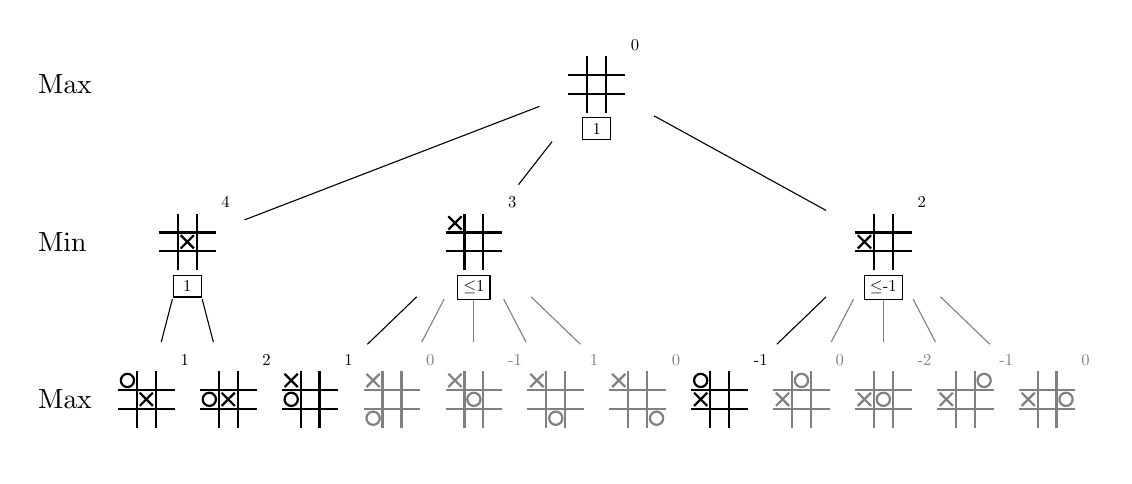
\begin{tikzpicture}[board/.style={minimum width=12*\s cm,minimum height=12*\s cm},eval/.style={anchor=south west,scale=5*\s},minmax/.style={draw=black,rectangle,anchor=north,scale=5*\s,minimum width=5*\s cm}]
\def\s{0.12};
\def\dx{1.04 cm};
\def\dy{-2 cm};
\draw (-1.5,0) node[anchor=west]{Max};
\draw (-1.5,\dy) node[anchor=west]{Min};
\draw (-1.5,2*\dy) node[anchor=west]{Max};

\node[board] (S) at (5.5*\dx,0) {};
\node[board] (SA) at (0.5*\dx,\dy) {};
\node[board] (SAA) at (0,2*\dy) {};
\node[board] (SAB) at (\dx,2*\dy) {};
\node[board] (SB) at (4*\dx,\dy) {};
\node[board] (SBA) at (2*\dx,2*\dy) {};
\node[board] (SBB) at (3*\dx,2*\dy) {};
\node[board] (SBC) at (4*\dx,2*\dy) {};
\node[board] (SBD) at (5*\dx,2*\dy) {};
\node[board] (SBE) at (6*\dx,2*\dy) {};
\node[board] (SC) at (9*\dx,\dy) {};
\node[board] (SCA) at (7*\dx,2*\dy) {};
\node[board] (SCB) at (8*\dx,2*\dy) {};
\node[board] (SCC) at (9*\dx,2*\dy) {};
\node[board] (SCD) at (10*\dx,2*\dy) {};
\node[board] (SCE) at (11*\dx,2*\dy) {};

\draw (S) -- (SA);
\draw (SA) -- (SAA);
\draw (SA) -- (SAB);
\draw (S) -- (SB);
\draw (SB) -- (SBA);
\draw[gray] (SB) -- (SBB);
\draw[gray] (SB) -- (SBC);
\draw[gray] (SB) -- (SBD);
\draw[gray] (SB) -- (SBE);
\draw (S) -- (SC);
\draw (SC) -- (SCA);
\draw[gray] (SC) -- (SCB);
\draw[gray] (SC) -- (SCC);
\draw[gray] (SC) -- (SCD);
\draw[gray] (SC) -- (SCE);

\begin{scope}[xshift=5.5*\dx,yshift=0]
 \draw[thick] (-3*\s,-\s) -- (3*\s,-\s);
 \draw[thick] (-3*\s,\s) -- (3*\s,\s);
 \draw[thick] (-\s,-3*\s) -- (-\s,3*\s);
 \draw[thick] (\s,-3*\s) -- (\s,3*\s);
 \draw (3*\s,3*\s) node[eval]{0};
 \draw (0,-3.5*\s) node[minmax]{1};
\end{scope}

\begin{scope}[xshift=0.5*\dx,yshift=\dy]
 \draw[thick] (-3*\s,-\s) -- (3*\s,-\s);
 \draw[thick] (-3*\s,\s) -- (3*\s,\s);
 \draw[thick] (-\s,-3*\s) -- (-\s,3*\s);
 \draw[thick] (\s,-3*\s) -- (\s,3*\s);
 \draw (3*\s,3*\s) node[eval]{4};
 \foreach\x/\y in {0/0} {
  \draw[thick] (-0.7*\s+2*\s*\x,-0.7*\s-2*\s*\y) -- (0.7*\s+2*\s*\x,0.7*\s-2*\s*\y);
  \draw[thick] (0.7*\s+2*\s*\x,-0.7*\s-2*\s*\y) -- (-0.7*\s+2*\s*\x,0.7*\s-2*\s*\y);
 }
 \draw (0,-3.5*\s) node[minmax]{1};
\end{scope}
\begin{scope}[xshift=4*\dx,yshift=\dy]
 \draw[thick] (-3*\s,-\s) -- (3*\s,-\s);
 \draw[thick] (-3*\s,\s) -- (3*\s,\s);
 \draw[thick] (-\s,-3*\s) -- (-\s,3*\s);
 \draw[thick] (\s,-3*\s) -- (\s,3*\s);
 \draw (3*\s,3*\s) node[eval]{3};
 \foreach\x/\y in {-1/-1} {
  \draw[thick] (-0.7*\s+2*\s*\x,-0.7*\s-2*\s*\y) -- (0.7*\s+2*\s*\x,0.7*\s-2*\s*\y);
  \draw[thick] (0.7*\s+2*\s*\x,-0.7*\s-2*\s*\y) -- (-0.7*\s+2*\s*\x,0.7*\s-2*\s*\y);
 }
 \draw (0,-3.5*\s) node[minmax]{$\leq$1};
\end{scope}
\begin{scope}[xshift=9*\dx,yshift=\dy]
 \draw[thick] (-3*\s,-\s) -- (3*\s,-\s);
 \draw[thick] (-3*\s,\s) -- (3*\s,\s);
 \draw[thick] (-\s,-3*\s) -- (-\s,3*\s);
 \draw[thick] (\s,-3*\s) -- (\s,3*\s);
 \draw (3*\s,3*\s) node[eval]{2};
 \foreach\x/\y in {-1/0} {
  \draw[thick] (-0.7*\s+2*\s*\x,-0.7*\s-2*\s*\y) -- (0.7*\s+2*\s*\x,0.7*\s-2*\s*\y);
  \draw[thick] (0.7*\s+2*\s*\x,-0.7*\s-2*\s*\y) -- (-0.7*\s+2*\s*\x,0.7*\s-2*\s*\y);
 }
 \draw (0,-3.5*\s) node[minmax]{$\leq$-1};
\end{scope}

\begin{scope}[xshift=0,yshift=2*\dy]
 \draw[thick] (-3*\s,-\s) -- (3*\s,-\s);
 \draw[thick] (-3*\s,\s) -- (3*\s,\s);
 \draw[thick] (-\s,-3*\s) -- (-\s,3*\s);
 \draw[thick] (\s,-3*\s) -- (\s,3*\s);
 \draw (3*\s,3*\s) node[eval]{1};
 \foreach\x/\y in {0/0} {
  \draw[thick] (-0.7*\s+2*\s*\x,-0.7*\s-2*\s*\y) -- (0.7*\s+2*\s*\x,0.7*\s-2*\s*\y);
  \draw[thick] (0.7*\s+2*\s*\x,-0.7*\s-2*\s*\y) -- (-0.7*\s+2*\s*\x,0.7*\s-2*\s*\y);
 }
 \foreach\x/\y in {-1/-1} {
  \draw[thick] (2*\s*\x,-2*\s*\y) circle (0.7*\s);
 }
\end{scope}
\begin{scope}[xshift=1*\dx,yshift=2*\dy]
 \draw[thick] (-3*\s,-\s) -- (3*\s,-\s);
 \draw[thick] (-3*\s,\s) -- (3*\s,\s);
 \draw[thick] (-\s,-3*\s) -- (-\s,3*\s);
 \draw[thick] (\s,-3*\s) -- (\s,3*\s);
 \draw (3*\s,3*\s) node[eval]{2};
 \foreach\x/\y in {0/0} {
  \draw[thick] (-0.7*\s+2*\s*\x,-0.7*\s-2*\s*\y) -- (0.7*\s+2*\s*\x,0.7*\s-2*\s*\y);
  \draw[thick] (0.7*\s+2*\s*\x,-0.7*\s-2*\s*\y) -- (-0.7*\s+2*\s*\x,0.7*\s-2*\s*\y);
 }
 \foreach\x/\y in {-1/0} {
  \draw[thick] (2*\s*\x,-2*\s*\y) circle (0.7*\s);
 }
\end{scope}
\begin{scope}[xshift=2*\dx,yshift=2*\dy]
 \draw[thick] (-3*\s,-\s) -- (3*\s,-\s);
 \draw[thick] (-3*\s,\s) -- (3*\s,\s);
 \draw[thick] (-\s,-3*\s) -- (-\s,3*\s);
 \draw[thick] (\s,-3*\s) -- (\s,3*\s);
 \draw (3*\s,3*\s) node[eval]{1};
 \foreach\x/\y in {-1/-1} {
  \draw[thick] (-0.7*\s+2*\s*\x,-0.7*\s-2*\s*\y) -- (0.7*\s+2*\s*\x,0.7*\s-2*\s*\y);
  \draw[thick] (0.7*\s+2*\s*\x,-0.7*\s-2*\s*\y) -- (-0.7*\s+2*\s*\x,0.7*\s-2*\s*\y);
 }
 \foreach\x/\y in {-1/0} {
  \draw[thick] (2*\s*\x,-2*\s*\y) circle (0.7*\s);
 }
\end{scope}
\begin{scope}[xshift=3*\dx,yshift=2*\dy,gray]
 \draw[thick] (-3*\s,-\s) -- (3*\s,-\s);
 \draw[thick] (-3*\s,\s) -- (3*\s,\s);
 \draw[thick] (-\s,-3*\s) -- (-\s,3*\s);
 \draw[thick] (\s,-3*\s) -- (\s,3*\s);
 \draw (3*\s,3*\s) node[eval]{0};
 \foreach\x/\y in {-1/-1} {
  \draw[thick] (-0.7*\s+2*\s*\x,-0.7*\s-2*\s*\y) -- (0.7*\s+2*\s*\x,0.7*\s-2*\s*\y);
  \draw[thick] (0.7*\s+2*\s*\x,-0.7*\s-2*\s*\y) -- (-0.7*\s+2*\s*\x,0.7*\s-2*\s*\y);
 }
 \foreach\x/\y in {-1/1} {
  \draw[thick] (2*\s*\x,-2*\s*\y) circle (0.7*\s);
 }
\end{scope}
\begin{scope}[xshift=4*\dx,yshift=2*\dy,gray]
 \draw[thick] (-3*\s,-\s) -- (3*\s,-\s);
 \draw[thick] (-3*\s,\s) -- (3*\s,\s);
 \draw[thick] (-\s,-3*\s) -- (-\s,3*\s);
 \draw[thick] (\s,-3*\s) -- (\s,3*\s);
 \draw (3*\s,3*\s) node[eval]{-1};
 \foreach\x/\y in {-1/-1} {
  \draw[thick] (-0.7*\s+2*\s*\x,-0.7*\s-2*\s*\y) -- (0.7*\s+2*\s*\x,0.7*\s-2*\s*\y);
  \draw[thick] (0.7*\s+2*\s*\x,-0.7*\s-2*\s*\y) -- (-0.7*\s+2*\s*\x,0.7*\s-2*\s*\y);
 }
 \foreach\x/\y in {0/0} {
  \draw[thick] (2*\s*\x,-2*\s*\y) circle (0.7*\s);
 }
\end{scope}
\begin{scope}[xshift=5*\dx,yshift=2*\dy,gray]
 \draw[thick] (-3*\s,-\s) -- (3*\s,-\s);
 \draw[thick] (-3*\s,\s) -- (3*\s,\s);
 \draw[thick] (-\s,-3*\s) -- (-\s,3*\s);
 \draw[thick] (\s,-3*\s) -- (\s,3*\s);
 \draw (3*\s,3*\s) node[eval]{1};
 \foreach\x/\y in {-1/-1} {
  \draw[thick] (-0.7*\s+2*\s*\x,-0.7*\s-2*\s*\y) -- (0.7*\s+2*\s*\x,0.7*\s-2*\s*\y);
  \draw[thick] (0.7*\s+2*\s*\x,-0.7*\s-2*\s*\y) -- (-0.7*\s+2*\s*\x,0.7*\s-2*\s*\y);
 }
 \foreach\x/\y in {0/1} {
  \draw[thick] (2*\s*\x,-2*\s*\y) circle (0.7*\s);
 }
\end{scope}
\begin{scope}[xshift=6*\dx,yshift=2*\dy,gray]
 \draw[thick] (-3*\s,-\s) -- (3*\s,-\s);
 \draw[thick] (-3*\s,\s) -- (3*\s,\s);
 \draw[thick] (-\s,-3*\s) -- (-\s,3*\s);
 \draw[thick] (\s,-3*\s) -- (\s,3*\s);
 \draw (3*\s,3*\s) node[eval]{0};
 \foreach\x/\y in {-1/-1} {
  \draw[thick] (-0.7*\s+2*\s*\x,-0.7*\s-2*\s*\y) -- (0.7*\s+2*\s*\x,0.7*\s-2*\s*\y);
  \draw[thick] (0.7*\s+2*\s*\x,-0.7*\s-2*\s*\y) -- (-0.7*\s+2*\s*\x,0.7*\s-2*\s*\y);
 }
 \foreach\x/\y in {1/1} {
  \draw[thick] (2*\s*\x,-2*\s*\y) circle (0.7*\s);
 }
\end{scope}
\begin{scope}[xshift=7*\dx,yshift=2*\dy]
 \draw[thick] (-3*\s,-\s) -- (3*\s,-\s);
 \draw[thick] (-3*\s,\s) -- (3*\s,\s);
 \draw[thick] (-\s,-3*\s) -- (-\s,3*\s);
 \draw[thick] (\s,-3*\s) -- (\s,3*\s);
 \draw (3*\s,3*\s) node[eval]{-1};
 \foreach\x/\y in {-1/0} {
  \draw[thick] (-0.7*\s+2*\s*\x,-0.7*\s-2*\s*\y) -- (0.7*\s+2*\s*\x,0.7*\s-2*\s*\y);
  \draw[thick] (0.7*\s+2*\s*\x,-0.7*\s-2*\s*\y) -- (-0.7*\s+2*\s*\x,0.7*\s-2*\s*\y);
 }
 \foreach\x/\y in {-1/-1} {
  \draw[thick] (2*\s*\x,-2*\s*\y) circle (0.7*\s);
 }
\end{scope}
\begin{scope}[xshift=8*\dx,yshift=2*\dy,gray]
 \draw[thick] (-3*\s,-\s) -- (3*\s,-\s);
 \draw[thick] (-3*\s,\s) -- (3*\s,\s);
 \draw[thick] (-\s,-3*\s) -- (-\s,3*\s);
 \draw[thick] (\s,-3*\s) -- (\s,3*\s);
 \draw (3*\s,3*\s) node[eval]{0};
 \foreach\x/\y in {-1/0} {
  \draw[thick] (-0.7*\s+2*\s*\x,-0.7*\s-2*\s*\y) -- (0.7*\s+2*\s*\x,0.7*\s-2*\s*\y);
  \draw[thick] (0.7*\s+2*\s*\x,-0.7*\s-2*\s*\y) -- (-0.7*\s+2*\s*\x,0.7*\s-2*\s*\y);
 }
 \foreach\x/\y in {0/-1} {
  \draw[thick] (2*\s*\x,-2*\s*\y) circle (0.7*\s);
 }
\end{scope}
\begin{scope}[xshift=9*\dx,yshift=2*\dy,gray]
 \draw[thick] (-3*\s,-\s) -- (3*\s,-\s);
 \draw[thick] (-3*\s,\s) -- (3*\s,\s);
 \draw[thick] (-\s,-3*\s) -- (-\s,3*\s);
 \draw[thick] (\s,-3*\s) -- (\s,3*\s);
 \draw (3*\s,3*\s) node[eval]{-2};
 \foreach\x/\y in {-1/0} {
  \draw[thick] (-0.7*\s+2*\s*\x,-0.7*\s-2*\s*\y) -- (0.7*\s+2*\s*\x,0.7*\s-2*\s*\y);
  \draw[thick] (0.7*\s+2*\s*\x,-0.7*\s-2*\s*\y) -- (-0.7*\s+2*\s*\x,0.7*\s-2*\s*\y);
 }
 \foreach\x/\y in {0/0} {
  \draw[thick] (2*\s*\x,-2*\s*\y) circle (0.7*\s);
 }
\end{scope}
\begin{scope}[xshift=10*\dx,yshift=2*\dy,gray]
 \draw[thick] (-3*\s,-\s) -- (3*\s,-\s);
 \draw[thick] (-3*\s,\s) -- (3*\s,\s);
 \draw[thick] (-\s,-3*\s) -- (-\s,3*\s);
 \draw[thick] (\s,-3*\s) -- (\s,3*\s);
 \draw (3*\s,3*\s) node[eval]{-1};
 \foreach\x/\y in {-1/0} {
  \draw[thick] (-0.7*\s+2*\s*\x,-0.7*\s-2*\s*\y) -- (0.7*\s+2*\s*\x,0.7*\s-2*\s*\y);
  \draw[thick] (0.7*\s+2*\s*\x,-0.7*\s-2*\s*\y) -- (-0.7*\s+2*\s*\x,0.7*\s-2*\s*\y);
 }
 \foreach\x/\y in {1/-1} {
  \draw[thick] (2*\s*\x,-2*\s*\y) circle (0.7*\s);
 }
\end{scope}
\begin{scope}[xshift=11*\dx,yshift=2*\dy,gray]
 \draw[thick] (-3*\s,-\s) -- (3*\s,-\s);
 \draw[thick] (-3*\s,\s) -- (3*\s,\s);
 \draw[thick] (-\s,-3*\s) -- (-\s,3*\s);
 \draw[thick] (\s,-3*\s) -- (\s,3*\s);
 \draw (3*\s,3*\s) node[eval]{0};
 \foreach\x/\y in {-1/0} {
  \draw[thick] (-0.7*\s+2*\s*\x,-0.7*\s-2*\s*\y) -- (0.7*\s+2*\s*\x,0.7*\s-2*\s*\y);
  \draw[thick] (0.7*\s+2*\s*\x,-0.7*\s-2*\s*\y) -- (-0.7*\s+2*\s*\x,0.7*\s-2*\s*\y);
 }
 \foreach\x/\y in {1/0} {
  \draw[thick] (2*\s*\x,-2*\s*\y) circle (0.7*\s);
 }
\end{scope}
\end{tikzpicture}
\caption{Een voorbeeld van beta-cuts bij Tic-Tac-Toe.}
\label{fig:betaCutTicTacToe}
\end{figure}
\subsection{Het Horizon-effect} 
Een groot nadeel aan het opbouwen van een boom die op een bepaalde diepte stopt is het \termen{Horizon-effect}. Dit effect stelt dat we volledig blind zijn voor wat onder de diepte-grens gebeurt. Vooral bij strategische spellen kunnen dergelijke effect nefast zijn: posities die er de eerste 4 zetten goed uitzien kunnen uiteindelijk tot een catastrofe leiden. Een oplossing bied het \termen{Heuristic Continuation}-principe. Dit principe stelt dat we bepaalde paden die er tot aan de horizon goed uitzien, beter verder onderzoeken. Dit privellege wordt alleen verleent aan paden die ofwel aan de horizon tot \'e\'en van de beste behoren, of waarbij een heuristiek alarmeert voor een strategisch belangrijke fase (bijvoorbeeld onmiddellijk stukkenverlies, koning in gevaar,...)
\paragraph{}
%Hoe wordt een dergelijke Heuristic Continuation dan georganiseerd? Een oplossing hiervoor is \termen{Tapering Search}. Hierbij stellen we opnieuw een diepte-limiet in. In plaats van echter alle paden te evalueren tot aan deze limiet wordt telkens een evaluatie gemaakt van alle kinderen. Afhankelijk van de rang die een bepaald kind inneemt krijgt het meer of minder recht op extra dieptes. Zo zal de topknoop haar beste kind beoordelen met een evaluatie tot aan die diepte-limiet. Het tweede kind met een evaluatie die afloopt op $1$ niveau van de dieptelimiet, enzovoort. Deze kinderen op hun beurt geven vervolgens opnieuw rechten aan hun kinderen. Hun beste kind geven ze dan hun eigen limiet verminderd met \'e\'en, enzovoort. Het slechtste kind wordt nooit verder ge\"evalueerd.??
Hoe wordt een dergelijke Heuristic Continuation dan georganiseerd? Een oplossing hiervoor is \termen{Tapering Search}. Hierbij evalueren we een knoop, met een zekere interne diepte-limiet. Vervolgens generen we de kinderen van deze knoop, en sorteren ze op hun evaluatie. Het beste kind erft vervolgens de diepte limiet over van zijn ouder vermindert met 1. Het tweede beste kind met een vermindering met twee, enzovoort tot de dieptelimiet 0 bedraagt. Deze methode roepen we dan ook aan startend vanuit de huidige toestand met over het algemeen een grote diepte limiet. Dit wordt formeel beschreven in \algref{alg:taperingSearch}.
\begin{algorithm}[htb]                      % enter the algorithm environment
\caption{$\mathcommand{taperingSearch}{\mbox{state},\depth,\depthbound}$}          % give the algorithm a caption
\label{alg:taperingSearch}                           % and a label for \ref{} commands later in the document
\begin{algorithmic}[1]                    % enter the algorithmic environment
\IF{$\depth<\depthbound$}
\STATE\COMMENT{Einde nog niet bereikt}
\STATE $C\leftarrow\mathcommand{children}{\mbox{state}}$
\STATE $\quicksort{C,\mathcommand{eval}{C_i}}$
\FOR{$i=0$ to $\minM{}{\#C,\depthbound}-1$}
\STATE $\mathcommand{taperingSearch}{R\left[i\right],\depth+1,\depthbound-1-i}$
\ENDFOR
\ENDIF
\end{algorithmic}
\end{algorithm}
\begin{leftbar}
Bij wijze van voorbeeld passen we Tapering Search toe bij Tic-Tac-Toe met een begindiepte van $d=3$. Zoals te zien op figuur \ref{fig:taperingSearchTicTacToe}. We expanderen eerst de eerste knoop, hierbij zien we dat bij $X$ in het midden we de beste evaluatiefunctie bekomen. Deze knoop zullen we dus verder expanderen met een diepte $d'=2$. Bij $X$ in een hoek bekomen we ook een goede heuristiek. Deze knoop expanderen we met $d'=1$. Tenslotte expanderen we het bord met $X$ aan een rand niet meer verder. Op analoge manier expanderen we vervolgens de onderliggende knopen.
\end{leftbar}
\begin{figure}[htb]
\centering
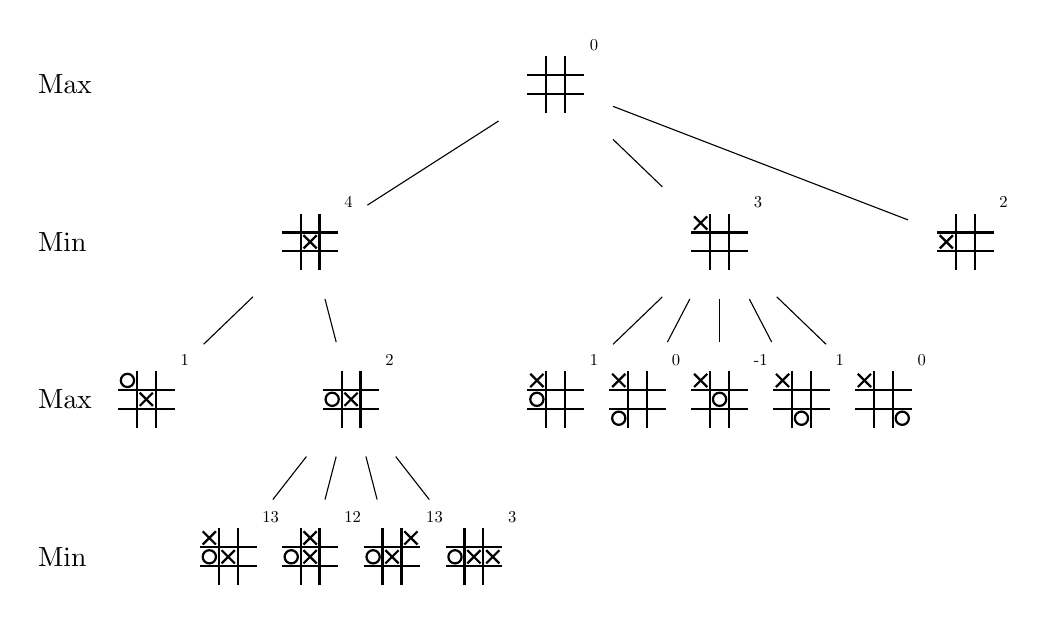
\begin{tikzpicture}[board/.style={minimum width=12*\s cm,minimum height=12*\s cm},eval/.style={anchor=south west,scale=5*\s},minmax/.style={draw=black,rectangle,anchor=north,scale=5*\s,minimum width=5*\s cm}]
\def\s{0.12};
\def\dx{1.04 cm};
\def\dy{-2 cm};
\draw (-1.5,0) node[anchor=west]{Max};
\draw (-1.5,\dy) node[anchor=west]{Min};
\draw (-1.5,2*\dy) node[anchor=west]{Max};
\draw (-1.5,3*\dy) node[anchor=west]{Min};

\node[board] (S) at (5*\dx,0) {};
\node[board] (SA) at (2*\dx,\dy) {};
\node[board] (SAA) at (0,2*\dy) {};
\node[board] (SAB) at (2.5*\dx,2*\dy) {};
\node[board] (SABA) at (1*\dx,3*\dy) {};
\node[board] (SABB) at (2*\dx,3*\dy) {};
\node[board] (SABC) at (3*\dx,3*\dy) {};
\node[board] (SABD) at (4*\dx,3*\dy) {};
\node[board] (SB) at (7*\dx,\dy) {};
\node[board] (SBA) at (5*\dx,2*\dy) {};
\node[board] (SBB) at (6*\dx,2*\dy) {};
\node[board] (SBC) at (7*\dx,2*\dy) {};
\node[board] (SBD) at (8*\dx,2*\dy) {};
\node[board] (SBE) at (9*\dx,2*\dy) {};
\node[board] (SC) at (10*\dx,\dy) {};

\draw (S) -- (SA);
\draw (SA) -- (SAA);
\draw (SA) -- (SAB);
\draw (SAB) -- (SABA);
\draw (SAB) -- (SABB);
\draw (SAB) -- (SABC);
\draw (SAB) -- (SABD);
\draw (S) -- (SB);
\draw (SB) -- (SBA);
\draw (SB) -- (SBB);
\draw (SB) -- (SBC);
\draw (SB) -- (SBD);
\draw (SB) -- (SBE);
\draw (S) -- (SC);

\begin{scope}[xshift=5*\dx,yshift=0]
 \draw[thick] (-3*\s,-\s) -- (3*\s,-\s);
 \draw[thick] (-3*\s,\s) -- (3*\s,\s);
 \draw[thick] (-\s,-3*\s) -- (-\s,3*\s);
 \draw[thick] (\s,-3*\s) -- (\s,3*\s);
 \draw (3*\s,3*\s) node[eval]{0};
 %\draw (0,-3.5*\s) node[minmax]{1};
\end{scope}

\begin{scope}[xshift=2*\dx,yshift=\dy]
 \draw[thick] (-3*\s,-\s) -- (3*\s,-\s);
 \draw[thick] (-3*\s,\s) -- (3*\s,\s);
 \draw[thick] (-\s,-3*\s) -- (-\s,3*\s);
 \draw[thick] (\s,-3*\s) -- (\s,3*\s);
 \draw (3*\s,3*\s) node[eval]{4};
 \foreach\x/\y in {0/0} {
  \draw[thick] (-0.7*\s+2*\s*\x,-0.7*\s-2*\s*\y) -- (0.7*\s+2*\s*\x,0.7*\s-2*\s*\y);
  \draw[thick] (0.7*\s+2*\s*\x,-0.7*\s-2*\s*\y) -- (-0.7*\s+2*\s*\x,0.7*\s-2*\s*\y);
 }
 %\draw (0,-3.5*\s) node[minmax]{1};
\end{scope}
\begin{scope}[xshift=7*\dx,yshift=\dy]
 \draw[thick] (-3*\s,-\s) -- (3*\s,-\s);
 \draw[thick] (-3*\s,\s) -- (3*\s,\s);
 \draw[thick] (-\s,-3*\s) -- (-\s,3*\s);
 \draw[thick] (\s,-3*\s) -- (\s,3*\s);
 \draw (3*\s,3*\s) node[eval]{3};
 \foreach\x/\y in {-1/-1} {
  \draw[thick] (-0.7*\s+2*\s*\x,-0.7*\s-2*\s*\y) -- (0.7*\s+2*\s*\x,0.7*\s-2*\s*\y);
  \draw[thick] (0.7*\s+2*\s*\x,-0.7*\s-2*\s*\y) -- (-0.7*\s+2*\s*\x,0.7*\s-2*\s*\y);
 }
 %\draw (0,-3.5*\s) node[minmax]{$\leq$1};
\end{scope}
\begin{scope}[xshift=10*\dx,yshift=\dy]
 \draw[thick] (-3*\s,-\s) -- (3*\s,-\s);
 \draw[thick] (-3*\s,\s) -- (3*\s,\s);
 \draw[thick] (-\s,-3*\s) -- (-\s,3*\s);
 \draw[thick] (\s,-3*\s) -- (\s,3*\s);
 \draw (3*\s,3*\s) node[eval]{2};
 \foreach\x/\y in {-1/0} {
  \draw[thick] (-0.7*\s+2*\s*\x,-0.7*\s-2*\s*\y) -- (0.7*\s+2*\s*\x,0.7*\s-2*\s*\y);
  \draw[thick] (0.7*\s+2*\s*\x,-0.7*\s-2*\s*\y) -- (-0.7*\s+2*\s*\x,0.7*\s-2*\s*\y);
 }
 %\draw (0,-3.5*\s) node[minmax]{$\leq$-1};
\end{scope}

\begin{scope}[xshift=0,yshift=2*\dy]
 \draw[thick] (-3*\s,-\s) -- (3*\s,-\s);
 \draw[thick] (-3*\s,\s) -- (3*\s,\s);
 \draw[thick] (-\s,-3*\s) -- (-\s,3*\s);
 \draw[thick] (\s,-3*\s) -- (\s,3*\s);
 \draw (3*\s,3*\s) node[eval]{1};
 \foreach\x/\y in {0/0} {
  \draw[thick] (-0.7*\s+2*\s*\x,-0.7*\s-2*\s*\y) -- (0.7*\s+2*\s*\x,0.7*\s-2*\s*\y);
  \draw[thick] (0.7*\s+2*\s*\x,-0.7*\s-2*\s*\y) -- (-0.7*\s+2*\s*\x,0.7*\s-2*\s*\y);
 }
 \foreach\x/\y in {-1/-1} {
  \draw[thick] (2*\s*\x,-2*\s*\y) circle (0.7*\s);
 }
\end{scope}
\begin{scope}[xshift=2.5*\dx,yshift=2*\dy]
 \draw[thick] (-3*\s,-\s) -- (3*\s,-\s);
 \draw[thick] (-3*\s,\s) -- (3*\s,\s);
 \draw[thick] (-\s,-3*\s) -- (-\s,3*\s);
 \draw[thick] (\s,-3*\s) -- (\s,3*\s);
 \draw (3*\s,3*\s) node[eval]{2};
 \foreach\x/\y in {0/0} {
  \draw[thick] (-0.7*\s+2*\s*\x,-0.7*\s-2*\s*\y) -- (0.7*\s+2*\s*\x,0.7*\s-2*\s*\y);
  \draw[thick] (0.7*\s+2*\s*\x,-0.7*\s-2*\s*\y) -- (-0.7*\s+2*\s*\x,0.7*\s-2*\s*\y);
 }
 \foreach\x/\y in {-1/0} {
  \draw[thick] (2*\s*\x,-2*\s*\y) circle (0.7*\s);
 }
\end{scope}
\begin{scope}[xshift=5*\dx,yshift=2*\dy]
 \draw[thick] (-3*\s,-\s) -- (3*\s,-\s);
 \draw[thick] (-3*\s,\s) -- (3*\s,\s);
 \draw[thick] (-\s,-3*\s) -- (-\s,3*\s);
 \draw[thick] (\s,-3*\s) -- (\s,3*\s);
 \draw (3*\s,3*\s) node[eval]{1};
 \foreach\x/\y in {-1/-1} {
  \draw[thick] (-0.7*\s+2*\s*\x,-0.7*\s-2*\s*\y) -- (0.7*\s+2*\s*\x,0.7*\s-2*\s*\y);
  \draw[thick] (0.7*\s+2*\s*\x,-0.7*\s-2*\s*\y) -- (-0.7*\s+2*\s*\x,0.7*\s-2*\s*\y);
 }
 \foreach\x/\y in {-1/0} {
  \draw[thick] (2*\s*\x,-2*\s*\y) circle (0.7*\s);
 }
\end{scope}
\begin{scope}[xshift=6*\dx,yshift=2*\dy]
 \draw[thick] (-3*\s,-\s) -- (3*\s,-\s);
 \draw[thick] (-3*\s,\s) -- (3*\s,\s);
 \draw[thick] (-\s,-3*\s) -- (-\s,3*\s);
 \draw[thick] (\s,-3*\s) -- (\s,3*\s);
 \draw (3*\s,3*\s) node[eval]{0};
 \foreach\x/\y in {-1/-1} {
  \draw[thick] (-0.7*\s+2*\s*\x,-0.7*\s-2*\s*\y) -- (0.7*\s+2*\s*\x,0.7*\s-2*\s*\y);
  \draw[thick] (0.7*\s+2*\s*\x,-0.7*\s-2*\s*\y) -- (-0.7*\s+2*\s*\x,0.7*\s-2*\s*\y);
 }
 \foreach\x/\y in {-1/1} {
  \draw[thick] (2*\s*\x,-2*\s*\y) circle (0.7*\s);
 }
\end{scope}
\begin{scope}[xshift=7*\dx,yshift=2*\dy]
 \draw[thick] (-3*\s,-\s) -- (3*\s,-\s);
 \draw[thick] (-3*\s,\s) -- (3*\s,\s);
 \draw[thick] (-\s,-3*\s) -- (-\s,3*\s);
 \draw[thick] (\s,-3*\s) -- (\s,3*\s);
 \draw (3*\s,3*\s) node[eval]{-1};
 \foreach\x/\y in {-1/-1} {
  \draw[thick] (-0.7*\s+2*\s*\x,-0.7*\s-2*\s*\y) -- (0.7*\s+2*\s*\x,0.7*\s-2*\s*\y);
  \draw[thick] (0.7*\s+2*\s*\x,-0.7*\s-2*\s*\y) -- (-0.7*\s+2*\s*\x,0.7*\s-2*\s*\y);
 }
 \foreach\x/\y in {0/0} {
  \draw[thick] (2*\s*\x,-2*\s*\y) circle (0.7*\s);
 }
\end{scope}
\begin{scope}[xshift=8*\dx,yshift=2*\dy]
 \draw[thick] (-3*\s,-\s) -- (3*\s,-\s);
 \draw[thick] (-3*\s,\s) -- (3*\s,\s);
 \draw[thick] (-\s,-3*\s) -- (-\s,3*\s);
 \draw[thick] (\s,-3*\s) -- (\s,3*\s);
 \draw (3*\s,3*\s) node[eval]{1};
 \foreach\x/\y in {-1/-1} {
  \draw[thick] (-0.7*\s+2*\s*\x,-0.7*\s-2*\s*\y) -- (0.7*\s+2*\s*\x,0.7*\s-2*\s*\y);
  \draw[thick] (0.7*\s+2*\s*\x,-0.7*\s-2*\s*\y) -- (-0.7*\s+2*\s*\x,0.7*\s-2*\s*\y);
 }
 \foreach\x/\y in {0/1} {
  \draw[thick] (2*\s*\x,-2*\s*\y) circle (0.7*\s);
 }
\end{scope}
\begin{scope}[xshift=9*\dx,yshift=2*\dy]
 \draw[thick] (-3*\s,-\s) -- (3*\s,-\s);
 \draw[thick] (-3*\s,\s) -- (3*\s,\s);
 \draw[thick] (-\s,-3*\s) -- (-\s,3*\s);
 \draw[thick] (\s,-3*\s) -- (\s,3*\s);
 \draw (3*\s,3*\s) node[eval]{0};
 \foreach\x/\y in {-1/-1} {
  \draw[thick] (-0.7*\s+2*\s*\x,-0.7*\s-2*\s*\y) -- (0.7*\s+2*\s*\x,0.7*\s-2*\s*\y);
  \draw[thick] (0.7*\s+2*\s*\x,-0.7*\s-2*\s*\y) -- (-0.7*\s+2*\s*\x,0.7*\s-2*\s*\y);
 }
 \foreach\x/\y in {1/1} {
  \draw[thick] (2*\s*\x,-2*\s*\y) circle (0.7*\s);
 }
\end{scope}
\begin{scope}[xshift=\dx,yshift=3*\dy]
 \draw[thick] (-3*\s,-\s) -- (3*\s,-\s);
 \draw[thick] (-3*\s,\s) -- (3*\s,\s);
 \draw[thick] (-\s,-3*\s) -- (-\s,3*\s);
 \draw[thick] (\s,-3*\s) -- (\s,3*\s);
 \draw (3*\s,3*\s) node[anchor=south west,scale=5*\s]{13};
 \foreach\x/\y in {-1/-1,0/0} {
  \draw[thick] (-0.7*\s+2*\s*\x,-0.7*\s-2*\s*\y) -- (0.7*\s+2*\s*\x,0.7*\s-2*\s*\y);
  \draw[thick] (0.7*\s+2*\s*\x,-0.7*\s-2*\s*\y) -- (-0.7*\s+2*\s*\x,0.7*\s-2*\s*\y);
 }
 \foreach\x/\y in {-1/0} {
  \draw[thick] (2*\s*\x,-2*\s*\y) circle (0.7*\s);
 }
\end{scope}
\begin{scope}[xshift=2*\dx,yshift=3*\dy]
 \draw[thick] (-3*\s,-\s) -- (3*\s,-\s);
 \draw[thick] (-3*\s,\s) -- (3*\s,\s);
 \draw[thick] (-\s,-3*\s) -- (-\s,3*\s);
 \draw[thick] (\s,-3*\s) -- (\s,3*\s);
 \draw (3*\s,3*\s) node[anchor=south west,scale=5*\s]{12};
 \foreach\x/\y in {0/-1,0/0} {
  \draw[thick] (-0.7*\s+2*\s*\x,-0.7*\s-2*\s*\y) -- (0.7*\s+2*\s*\x,0.7*\s-2*\s*\y);
  \draw[thick] (0.7*\s+2*\s*\x,-0.7*\s-2*\s*\y) -- (-0.7*\s+2*\s*\x,0.7*\s-2*\s*\y);
 }
 \foreach\x/\y in {-1/0} {
  \draw[thick] (2*\s*\x,-2*\s*\y) circle (0.7*\s);
 }
\end{scope}
\begin{scope}[xshift=3*\dx,yshift=3*\dy]
 \draw[thick] (-3*\s,-\s) -- (3*\s,-\s);
 \draw[thick] (-3*\s,\s) -- (3*\s,\s);
 \draw[thick] (-\s,-3*\s) -- (-\s,3*\s);
 \draw[thick] (\s,-3*\s) -- (\s,3*\s);
 \draw (3*\s,3*\s) node[anchor=south west,scale=5*\s]{13};
 \foreach\x/\y in {0/0,1/-1} {
  \draw[thick] (-0.7*\s+2*\s*\x,-0.7*\s-2*\s*\y) -- (0.7*\s+2*\s*\x,0.7*\s-2*\s*\y);
  \draw[thick] (0.7*\s+2*\s*\x,-0.7*\s-2*\s*\y) -- (-0.7*\s+2*\s*\x,0.7*\s-2*\s*\y);
 }
 \foreach\x/\y in {-1/0} {
  \draw[thick] (2*\s*\x,-2*\s*\y) circle (0.7*\s);
 }
\end{scope}
\begin{scope}[xshift=4*\dx,yshift=3*\dy]
 \draw[thick] (-3*\s,-\s) -- (3*\s,-\s);
 \draw[thick] (-3*\s,\s) -- (3*\s,\s);
 \draw[thick] (-\s,-3*\s) -- (-\s,3*\s);
 \draw[thick] (\s,-3*\s) -- (\s,3*\s);
 \draw (3*\s,3*\s) node[anchor=south west,scale=5*\s]{3};
 \foreach\x/\y in {0/0,1/0} {
  \draw[thick] (-0.7*\s+2*\s*\x,-0.7*\s-2*\s*\y) -- (0.7*\s+2*\s*\x,0.7*\s-2*\s*\y);
  \draw[thick] (0.7*\s+2*\s*\x,-0.7*\s-2*\s*\y) -- (-0.7*\s+2*\s*\x,0.7*\s-2*\s*\y);
 }
 \foreach\x/\y in {-1/0} {
  \draw[thick] (2*\s*\x,-2*\s*\y) circle (0.7*\s);
 }
\end{scope}
\end{tikzpicture}
\caption{Tapering Search met $d=3$ bij Tic-Tac-Toe.}
\label{fig:taperingSearchTicTacToe}
\end{figure}
\subsection{Tijdslimieten}
Zoeken met een diepte-limiet, is niet altijd de beste methode voor tijdsgebonden spelletjes. Dergelijke zoekmethodes kunnen immers erg vari\"eren in tijdsgebruik, men loopt dus de kans dat het algoritme nog geen oplossing heeft wanneer de tijd op is. Een oplossing biedt het Iterative Deepening concept. Hierbij wordt de dieptegrens telkens met een factor verhoogt. Indien we initieel een lage diepte-grens hanteren, hebben we meestal een eerste oplossing in een kwestie van milliseconden. Vervolgens verdiepen we, indien we hierbij tot een resultaat komen, zullen we dit accepteren als nieuwe oplossing. Indien de tijd verstreken is, retourneren we de oplossing van onze laatste diepte. Hierdoor hebben we altijd een oplossing klaar indien de tijd opraakt.
\subsection{Kansspelen}
Bij kansspelen is het verloop van het spel nog moeilijker te bepalen. In dat geval kunnen we de dobbelsteen of een andere toevalsgenerator, beschouwen als een derde speler. Deze speler krijgt vervolgens een aparte soort knopen toegewezen: \termen{expectimin-knopen} en \termen{expectimax-knopen}, afhankelijk van de plaats waar de dobbelsteen zich tussen de spelers bevindt (expectimax onder een maximum-knoop en expectimin-onder een minimum-knoop). Vervolgens zal deze knoop het gewogen gemiddelde van respectievelijk het minimum of het maximum van de knopen genereren, of meer formeel met $d_i$ de waarde van de toevalsgenerator:
\begin{equation}
\begin{array}{l}
\mathfunc{expectimin}{C}=\displaystyle\sum_{i}{P\left(d_i\right)\cdot\mbox{min}\left(\mathfunc{eval}{s}\right|\forall s\in\mathfunc{children}{d_i})}\\\\
\mathfunc{expectimax}{C}=\displaystyle\sum_{i}{P\left(d_i\right)\cdot\mbox{max}\left(\mathfunc{eval}{s}\right|\forall s\in\mathfunc{children}{d_i})}
\end{array}
\end{equation}